% !TEX root = ../entropy.tex

\section{Additional results}%
\label{sec:additional_results}

\subsection{Endogeneity}%
\label{sub:endogeneity}

As discussed in Section~\ref{sec:estimation}, one concern one might have about
our results in Section~\ref{sec:main_results} is reverse causality:
transferring money into savings accounts might change the distribution of spend
categories and thus change entropy. As noted previously, this is not a major
concern because of the way we calculate savings and spend profiles: savings are
calculated as the sum of inflows into savings accounts, while spend profiles
are based on the classification of spend transactions in current accounts, and
transfers from current to savings accounts are labelled as such and not treated
as spend transactions.

However, because transaction labelling is imperfect, it is possible that some
transfers are misclassified as spends and included in the calculation of
entropy scores. Two ways to deal with this is to use lagged entropy scores and
to explicitly control for the number of non-zero spend categories used to
calculate entropy scores. Here, we show that our results remain qualitatively
unchanged with both of these approaches.

Table~\ref{tab:reg_has_inflows_lag} presents results similar to the main
results in the main text, but using entropy lagged by one year-month period as
the independent variable of interest, while Table~\ref{tab:reg_has_inflows_cnz}
adds the number of non-zero spend categories as an additional control.

\def\yvars{has_inflows}
\foreach \y in \yvars {
    \input{\tabdir/reg_\y_cnz.tex}
    \input{\tabdir/reg_\y_lag.tex}
}


\subsection{Further results by financial resilience}%
\label{sub:results_by_financial_resilience}

The Tables below show results presented in
Section~\ref{sub:effect_of_financial_resilience} for alternative entropy
variables. 

\def\evars{entropy_tag, entropy_merchant}
\foreach \e in \evars {
    \input{\tabdir/reg_has_inflows_\e_z_inc_quint.tex}
    \input{\tabdir/reg_has_inflows_\e_sz_inc_quint.tex}
    \input{\tabdir/reg_has_inflows_\e_z_inc_var_quint.tex}
    \input{\tabdir/reg_has_inflows_\e_sz_inc_var_quint.tex}
}

% \subsection{Old stuff}%
% \label{sub:old_stuff}
% \newpage
% \subsection{Exploration}%
% \label{sub:exploration}
% 
\begin{table}[htbp]
   \centering
   \tiny
   \begin{threeparttable}[b]
      \caption{\label{tab:reg_has_sa_inflows_explore} Entropy exploration}
      \begin{tabular}{lccc}
         \tabularnewline \midrule \midrule
         Dependent Variable: & \multicolumn{3}{c}{Has savings}\\
         Model:                    & (1)             & (2)             & (3)\\  
         \midrule
         \emph{Variables}\\
         Entropy (48 cats)         &                 & 0.029$^{***}$   &   \\   
                                   &                 & [0.013; 0.044]  &   \\   
         Entropy (48 cats, smooth) &                 &                 & 0.004\\   
                                   &                 &                 & [-0.008; 0.016]\\   
         Spend txns                & 0.001$^{***}$   & 0.001$^{***}$   & 0.001$^{***}$\\   
                                   & [0.000; 0.001]  & [0.001; 0.001]  & [0.000; 0.001]\\   
         Unique categories         & 0.004$^{***}$   & 0.001           & 0.004$^{***}$\\   
                                   & [0.002; 0.006]  & [-0.002; 0.003] & [0.002; 0.006]\\   
         Paid with credit (\%)     & -0.000          & -0.000          & -0.000\\   
                                   & [-0.001; 0.000] & [-0.001; 0.000] & [-0.001; 0.000]\\   
         Month spend               & 0.006$^{***}$   & 0.005$^{***}$   & 0.006$^{***}$\\   
                                   & [0.003; 0.008]  & [0.003; 0.008]  & [0.003; 0.008]\\   
         Urban                     & -0.022          & -0.019          & -0.021\\   
                                   & [-0.230; 0.187] & [-0.230; 0.192] & [-0.230; 0.187]\\   
         Month income              & 0.000           & -0.000          & 0.000\\   
                                   & [-0.007; 0.007] & [-0.007; 0.006] & [-0.007; 0.007]\\   
         Has income in month       & 0.038$^{**}$    & 0.038$^{**}$    & 0.038$^{**}$\\   
                                   & [0.008; 0.068]  & [0.008; 0.068]  & [0.009; 0.068]\\   
         Income variability        & -0.003          & -0.003          & -0.003\\   
                                   & [-0.012; 0.006] & [-0.012; 0.005] & [-0.012; 0.005]\\   
         Rent payment              & 0.023$^{**}$    & 0.024$^{**}$    & 0.023$^{**}$\\   
                                   & [0.004; 0.043]  & [0.004; 0.043]  & [0.004; 0.043]\\   
         Mortgage payment          & 0.015           & 0.015           & 0.015\\   
                                   & [-0.009; 0.039] & [-0.009; 0.039] & [-0.009; 0.039]\\   
         Loan repayment            & 0.003           & 0.003           & 0.003\\   
                                   & [-0.013; 0.019] & [-0.012; 0.019] & [-0.013; 0.019]\\   
         Benefits                  & -0.010          & -0.011          & -0.010\\   
                                   & [-0.048; 0.028] & [-0.049; 0.027] & [-0.048; 0.028]\\   
         \midrule
         \emph{Fixed-effects}\\
         User id                   & Yes             & Yes             & Yes\\  
         Calendar month            & Yes             & Yes             & Yes\\  
         \midrule
         \emph{Fit statistics}\\
         Observations              & 83,935          & 83,935          & 83,935\\  
         R$^2$                     & 0.42912         & 0.42929         & 0.42913\\  
         Within R$^2$              & 0.00464         & 0.00494         & 0.00465\\  
         \midrule \midrule
         \multicolumn{4}{l}{\emph{Clustered (User id) co-variance matrix, 95\% confidence intervals in brackets}}\\
         \multicolumn{4}{l}{\emph{Signif. Codes: ***: 0.01, **: 0.05, *: 0.1}}\\
      \end{tabular}
      
      \begin{tablenotes}\footnotesize
         \item Notes: Spend and income variables are in \pounds'000.
      \end{tablenotes}
   \end{threeparttable}
\end{table}



\begin{table}[htbp]
   \centering
   \begin{threeparttable}[b]
      \caption{Components exploration}
      \begin{tabular}{lcccc}
         \tabularnewline \midrule \midrule
         Dependent Variable: & \multicolumn{4}{c}{Has savings}\\
         Model:                 & (1)             & (2)             & (3)              & (4)\\  
         \midrule
         \emph{Variables}\\
         Entropy (48 cats)      &                 & 0.032$^{***}$   &                  & 0.044$^{***}$\\   
                                &                 & [0.021; 0.042]  &                  & [0.024; 0.064]\\   
         Average spend          &                 &                 & 0.000$^{*}$      & 0.000$^{**}$\\   
                                &                 &                 & [-0.000; 0.000]  & [0.000; 0.000]\\   
         Cnz                    &                 &                 & 0.006$^{***}$    & 0.001\\   
                                &                 &                 & [0.004; 0.007]   & [-0.002; 0.003]\\   
         Counts std all         &                 &                 & 0.004$^{**}$     & 0.011$^{***}$\\   
                                &                 &                 & [0.001; 0.008]   & [0.006; 0.016]\\   
         Paid with credit (\%)  & -0.000          & -0.000          & -0.000$^{**}$    & -0.000$^{**}$\\   
                                & [-0.001; 0.000] & [-0.001; 0.000] & [-0.001; -0.000] & [-0.001; -0.000]\\   
         Month spend            & 0.020$^{***}$   & 0.019$^{***}$   & 0.015$^{***}$    & 0.014$^{***}$\\   
                                & [0.018; 0.023]  & [0.017; 0.022]  & [0.011; 0.019]   & [0.010; 0.018]\\   
         Urban                  & -0.039          & -0.037          & -0.037           & -0.036\\   
                                & [-0.230; 0.152] & [-0.234; 0.159] & [-0.233; 0.158]  & [-0.234; 0.163]\\   
         Month income           & 0.004           & 0.003           & 0.003            & 0.002\\   
                                & [-0.003; 0.011] & [-0.004; 0.010] & [-0.004; 0.009]  & [-0.005; 0.009]\\   
         Has income in month    & 0.039$^{**}$    & 0.037$^{**}$    & 0.032$^{**}$     & 0.031$^{*}$\\   
                                & [0.007; 0.071]  & [0.005; 0.069]  & [0.000; 0.064]   & [-0.000; 0.063]\\   
         Income variability     & 0.003           & 0.003           & 0.003            & 0.003\\   
                                & [-0.006; 0.012] & [-0.006; 0.012] & [-0.006; 0.011]  & [-0.006; 0.011]\\   
         Rent payment           & 0.028$^{***}$   & 0.025$^{***}$   & 0.023$^{**}$     & 0.023$^{**}$\\   
                                & [0.009; 0.047]  & [0.006; 0.043]  & [0.004; 0.041]   & [0.004; 0.042]\\   
         Mortgage payment       & 0.008           & 0.003           & -0.000           & -0.000\\   
                                & [-0.016; 0.033] & [-0.022; 0.027] & [-0.025; 0.024]  & [-0.025; 0.024]\\   
         Loan repayment         & 0.004           & -0.000          & -0.003           & -0.002\\   
                                & [-0.012; 0.020] & [-0.016; 0.016] & [-0.019; 0.013]  & [-0.018; 0.014]\\   
         Benefits               & -0.004          & -0.005          & -0.007           & -0.008\\   
                                & [-0.041; 0.033] & [-0.043; 0.032] & [-0.044; 0.030]  & [-0.045; 0.030]\\   
         \midrule
         \emph{Fixed-effects}\\
         User id                & Yes             & Yes             & Yes              & Yes\\  
         Calendar month         & Yes             & Yes             & Yes              & Yes\\  
         \midrule
         \emph{Fit statistics}\\
         Observations           & 91,644          & 91,644          & 91,644           & 91,644\\  
         R$^2$                  & 0.41730         & 0.41776         & 0.41807          & 0.41833\\  
         Within R$^2$           & 0.00782         & 0.00860         & 0.00914          & 0.00957\\  
         \midrule \midrule
         \multicolumn{5}{l}{\emph{Clustered (User id) co-variance matrix, 95\% confidence intervals in brackets}}\\
         \multicolumn{5}{l}{\emph{Signif. Codes: ***: 0.01, **: 0.05, *: 0.1}}\\
      \end{tabular}
   \end{threeparttable}
\end{table}



% 
\begin{table}[htbp]
   \centering
   \tiny
   \begin{threeparttable}[b]
      \caption{\label{tab:reg_has_sa_inflows_explore} Entropy exploration}
      \begin{tabular}{lccccc}
         \tabularnewline \midrule \midrule
         Dependent Variable: & \multicolumn{5}{c}{Entropy (48 cats)}\\
         Model:                    & (1)            & (2)            & (3)            & (4)              & (5)\\  
         \midrule
         \emph{Variables}\\
         Entropy (48 cats, smooth) & 0.274$^{***}$  &                &                &                  & 0.539$^{***}$\\   
                                   & [0.264; 0.285] &                &                &                  & [0.528; 0.550]\\   
         Spend txns                &                & 0.001$^{***}$  &                &                  & 0.010$^{***}$\\   
                                   &                & [0.001; 0.002] &                &                  & [0.010; 0.010]\\   
         Unique categories         &                &                & 0.097$^{***}$  &                  & 0.081$^{***}$\\   
                                   &                &                & [0.096; 0.099] &                  & [0.079; 0.082]\\   
         Category count variation  &                &                &                & -0.000$^{***}$   & -0.000$^{***}$\\   
                                   &                &                &                & [-0.000; -0.000] & [-0.000; -0.000]\\   
         \midrule
         \emph{Fixed-effects}\\
         User id                   & Yes            & Yes            & Yes            & Yes              & Yes\\  
         Calendar month            & Yes            & Yes            & Yes            & Yes              & Yes\\  
         \midrule
         \emph{Fit statistics}\\
         Observations              & 83,935         & 83,935         & 83,935         & 83,935           & 83,935\\  
         R$^2$                     & 0.66423        & 0.59311        & 0.77939        & 0.61808          & 0.92879\\  
         Within R$^2$              & 0.17916        & 0.00530        & 0.46067        & 0.06634          & 0.82592\\  
         \midrule \midrule
         \multicolumn{6}{l}{\emph{Clustered (User id) co-variance matrix, 95\% confidence intervals in brackets}}\\
         \multicolumn{6}{l}{\emph{Signif. Codes: ***: 0.01, **: 0.05, *: 0.1}}\\
      \end{tabular}
      
      \begin{tablenotes}\footnotesize
         \item Notes: Spend and income variables are in \pounds'000.
      \end{tablenotes}
   \end{threeparttable}
\end{table}



% 
\begin{table}[htbp]
   \centering
   \tiny
   \begin{threeparttable}[b]
      \caption{\label{tab:reg_has_sa_inflows_explore} Entropy exploration}
      \begin{tabular}{lccccc}
         \tabularnewline \midrule \midrule
         Dependent Variable: & \multicolumn{5}{c}{Entropy (48 cats)}\\
         Model:                    & (1)            & (2)            & (3)              & (4)              & (5)\\  
         \midrule
         \emph{Variables}\\
         Entropy (48 cats, smooth) & 0.212$^{***}$  &                &                  &                  & 0.530$^{***}$\\   
                                   & [0.208; 0.216] &                &                  &                  & [0.526; 0.533]\\   
         Spend txns                &                & 0.003$^{***}$  &                  &                  & 0.010$^{***}$\\   
                                   &                & [0.003; 0.003] &                  &                  & [0.010; 0.010]\\   
         Unique categories         &                &                & 0.098$^{***}$    &                  & 0.080$^{***}$\\   
                                   &                &                & [0.097; 0.098]   &                  & [0.080; 0.081]\\   
         Category count variation  &                &                &                  & -0.000$^{***}$   & -0.000$^{***}$\\   
                                   &                &                &                  & [-0.000; -0.000] & [-0.000; -0.000]\\   
         (Intercept)               & 0.501$^{***}$  & 0.213$^{***}$  & -1.079$^{***}$   & 0.508$^{***}$    & -1.228$^{***}$\\   
                                   & [0.497; 0.504] & [0.205; 0.221] & [-1.088; -1.069] & [0.503; 0.512]   & [-1.232; -1.223]\\   
         \midrule
         \emph{Fit statistics}\\
         Observations              & 83,935         & 83,935         & 83,935           & 83,935           & 83,935\\  
         R$^2$                     & 0.10447        & 0.04296        & 0.56104          & 0.02614          & 0.88513\\  
         Adjusted R$^2$            & 0.10446        & 0.04295        & 0.56104          & 0.02613          & 0.88513\\  
         \midrule \midrule
         \multicolumn{6}{l}{\emph{IID co-variance matrix, 95\% confidence intervals in brackets}}\\
         \multicolumn{6}{l}{\emph{Signif. Codes: ***: 0.01, **: 0.05, *: 0.1}}\\
      \end{tabular}
      
      \begin{tablenotes}\footnotesize
         \item Notes: Spend and income variables are in \pounds'000.
      \end{tablenotes}
   \end{threeparttable}
\end{table}



% % 
\begin{table}[htbp]
   \centering
   \tiny
   \begin{threeparttable}[b]
      \caption{\label{tab:reg_has_sa_inflows_explore} Entropy exploration}
      \begin{tabular}{lc}
         \tabularnewline \midrule \midrule
         Dependent Variable:       & Has savings\\  
         Model:                    & (1)\\  
         \midrule
         \emph{Variables}\\
         Entropy (48 cats, smooth) & -0.012$^{***}$\\   
                                   & [-0.016; -0.008]\\   
         (Intercept)               & 0.369$^{***}$\\   
                                   & [0.366; 0.373]\\   
         \midrule
         \emph{Fit statistics}\\
         Observations              & 83,935\\  
         R$^2$                     & 0.00040\\  
         Adjusted R$^2$            & 0.00039\\  
         \midrule \midrule
         \multicolumn{2}{l}{\emph{IID co-variance matrix, 95\% confidence intervals in brackets}}\\
         \multicolumn{2}{l}{\emph{Signif. Codes: ***: 0.01, **: 0.05, *: 0.1}}\\
      \end{tabular}
      
      \begin{tablenotes}\footnotesize
         \item Notes: Spend and income variables are in \pounds'000.
      \end{tablenotes}
   \end{threeparttable}
\end{table}




% \newpage
% \begin{figure}[H]
%     \caption{Diagnostics}
%     \label{fig:diagnostics}
%     \begin{center}
%         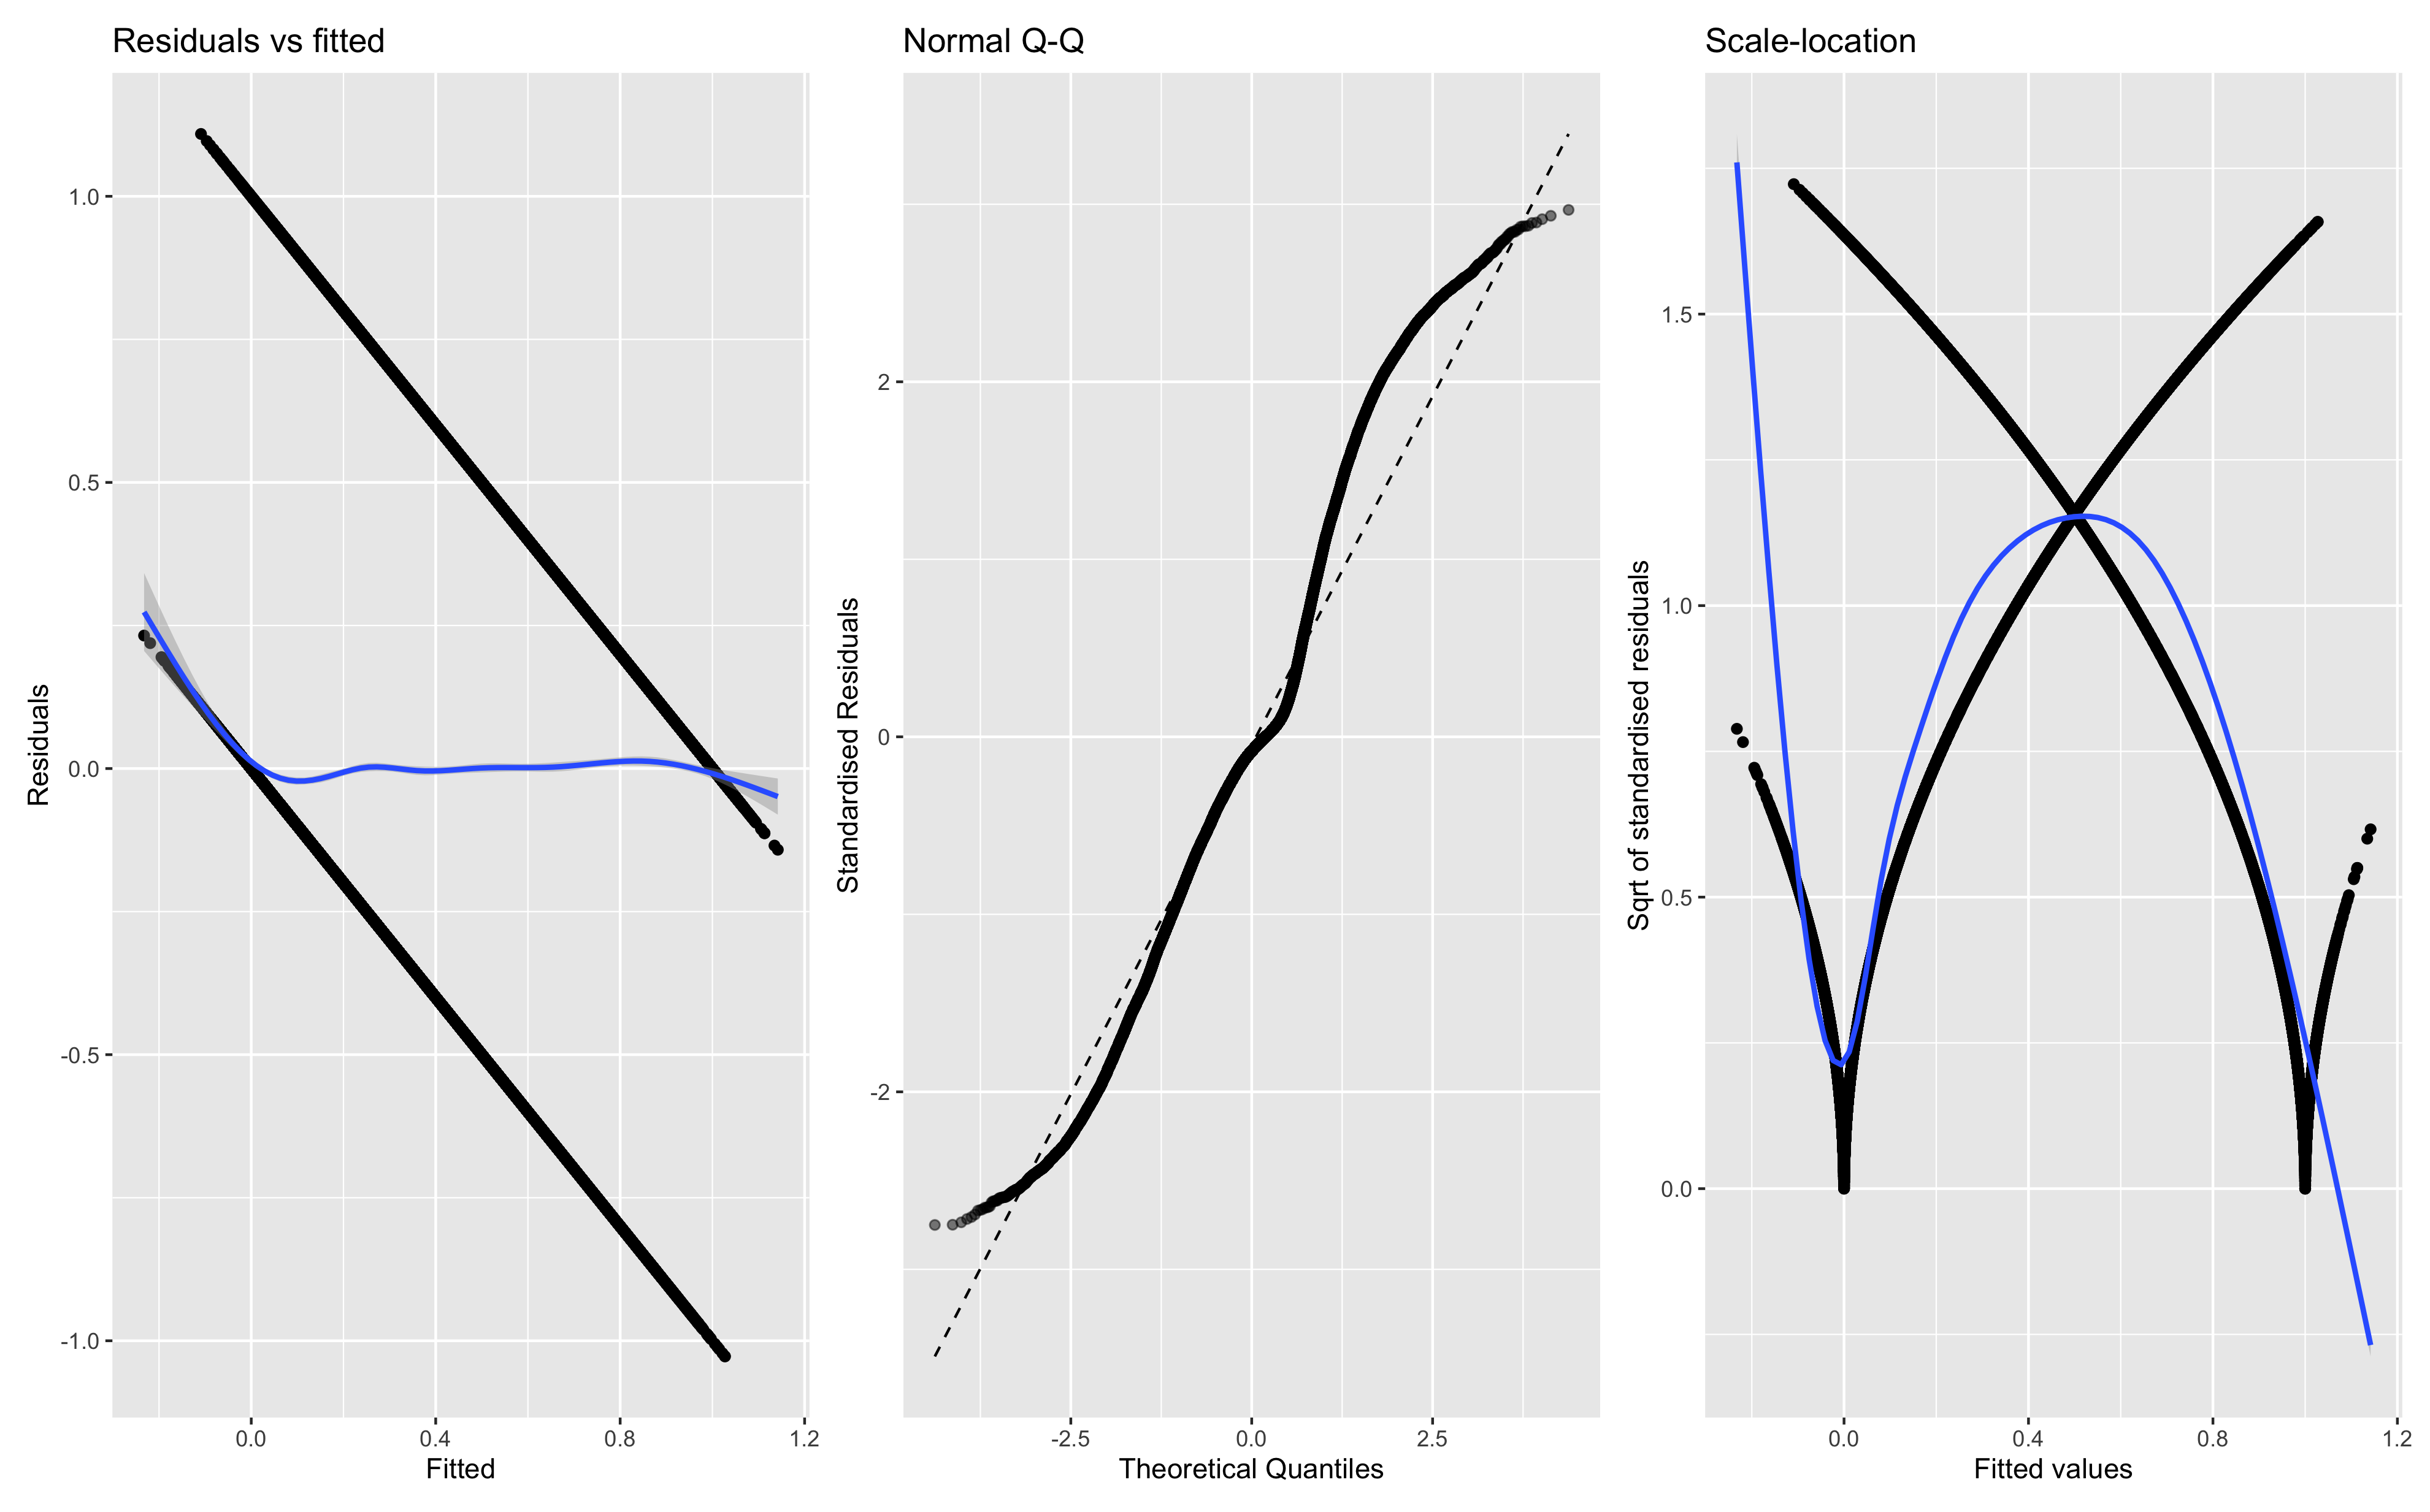
\includegraphics[width=0.9\textwidth]{\figdir/diagnostics.png}
%     \end{center}
% \end{figure}

% \newpage
% \begin{figure}[H]
%     \caption{Entropy and unique tags}
%     \label{fig:entropy_tag_vs_nunique}
%     \begin{center}
%         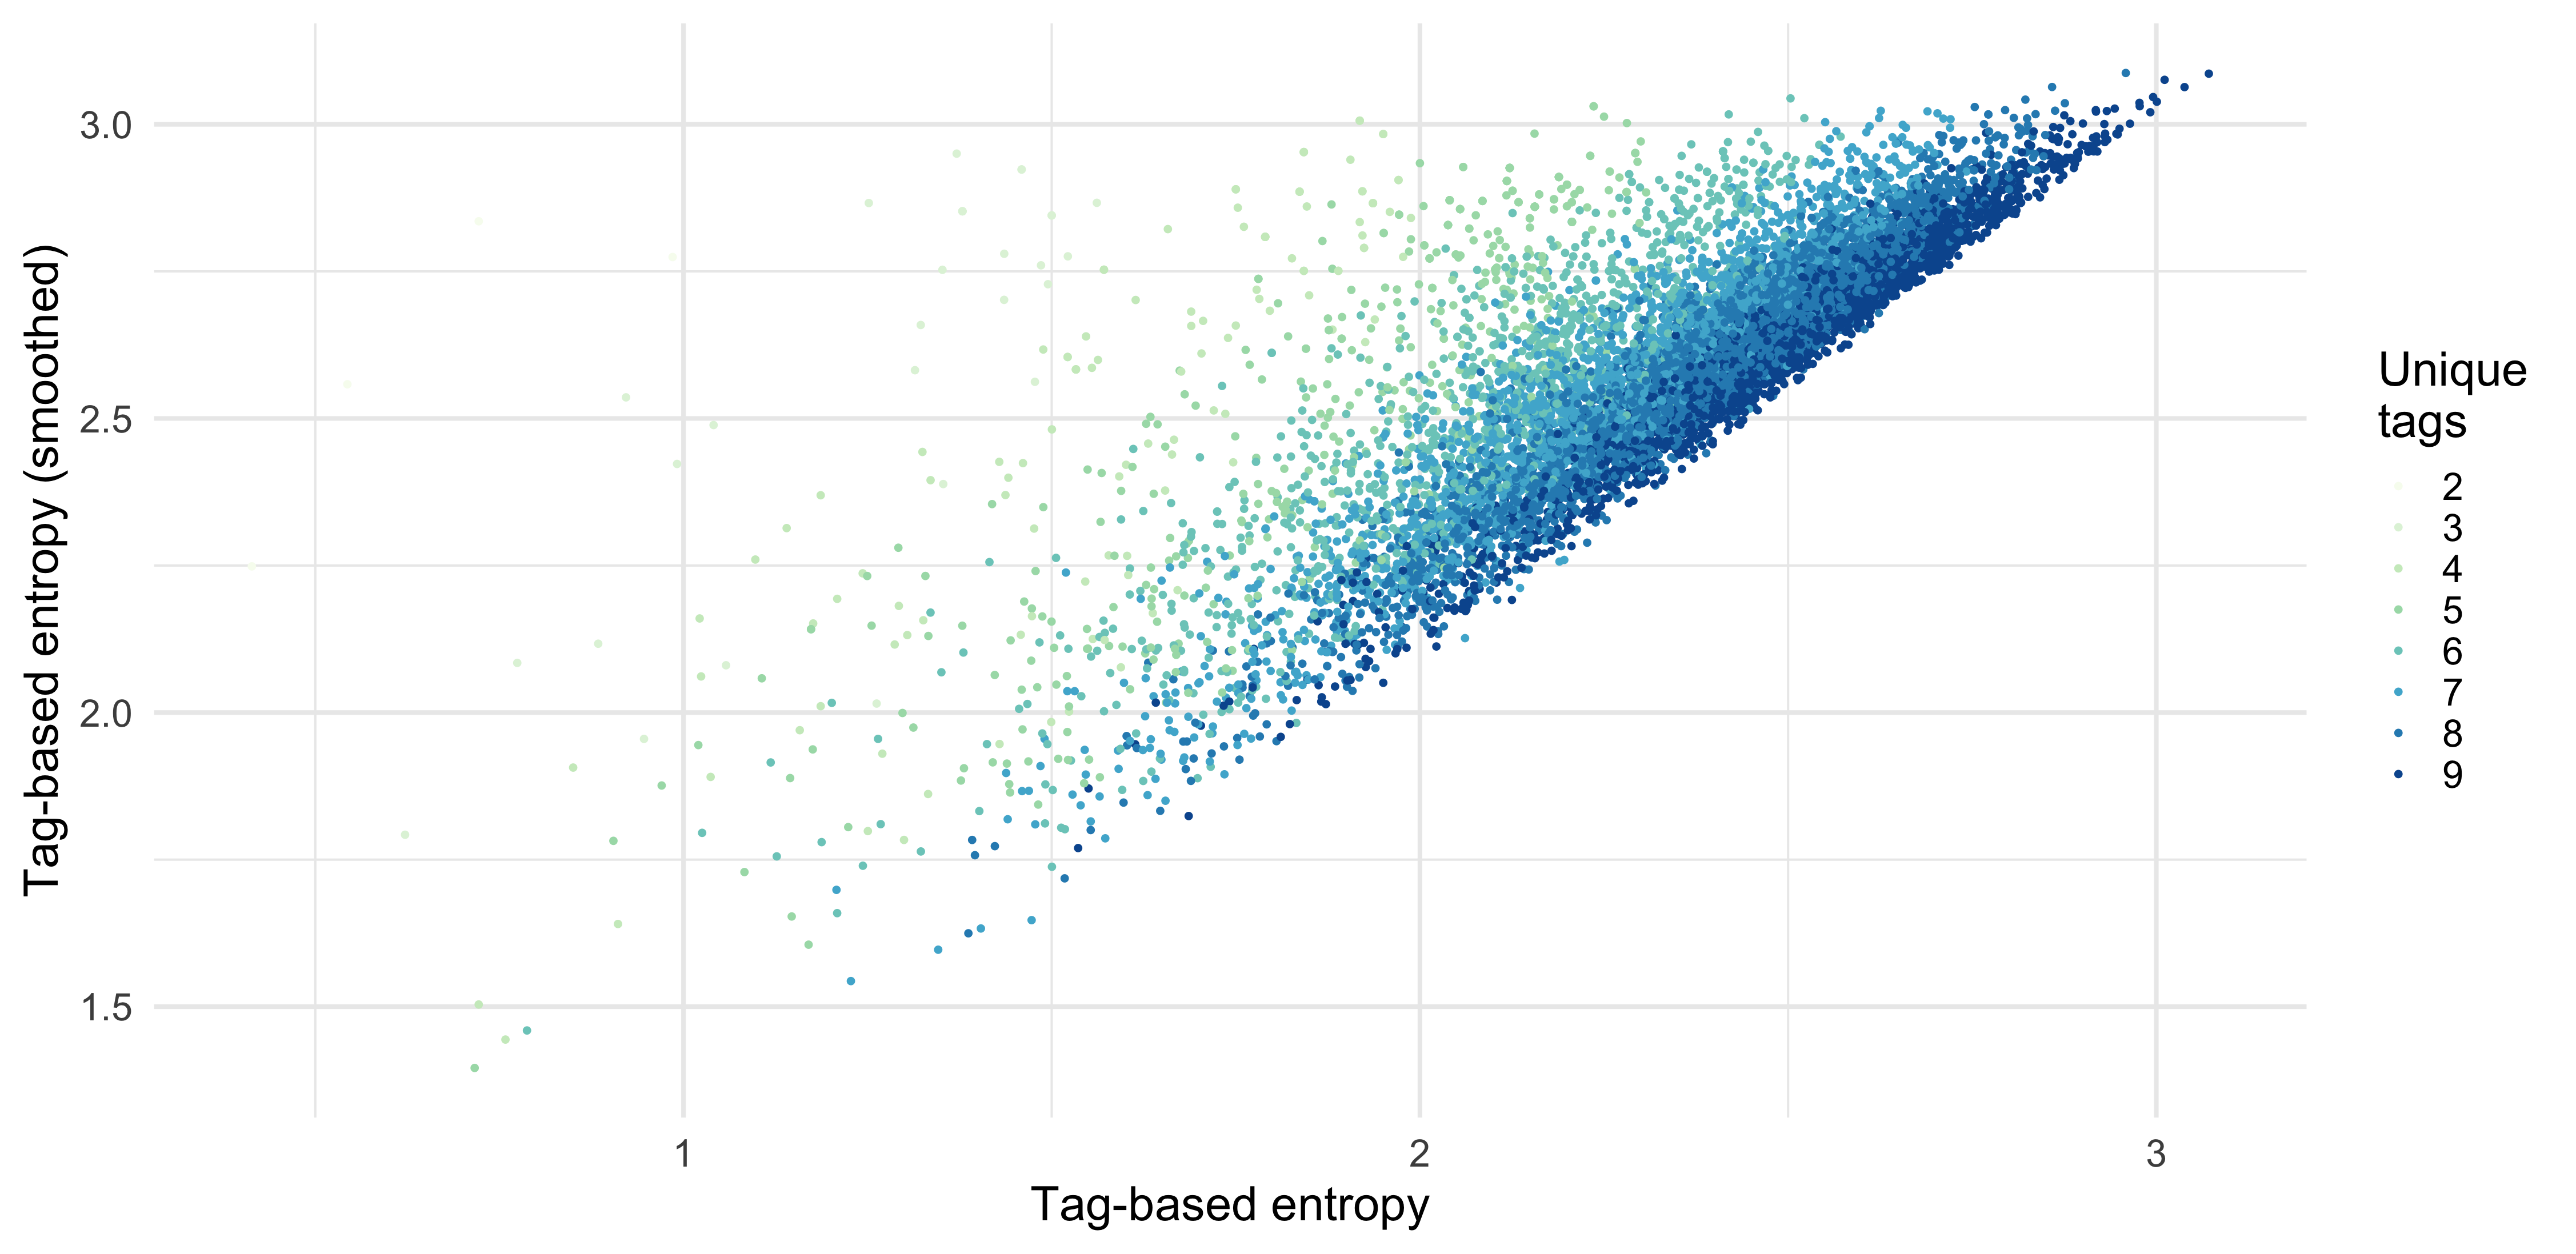
\includegraphics[width=0.9\textwidth]{\figdir/entropy_tag_vs_nunique.png}
%     \end{center}
% \end{figure}

